\subsection{Progettazione di dettaglio e codifica}
\textbf{Periodo}: dal \textbf{2022-02-20} al \textbf{2022-03-13} \mbox{} \\ \mbox{} \\

Le precondizioni sono:
\begin{itemize}
\item le postcondizioni della fase precedente sono state soddisfatte.
\end{itemize}

Le postcondizioni sono:
\begin{itemize}
\item aggiornamento e approvazione dei documenti prodotti precedentemente;
\item completamento codifica e verifica;
\item realizzazione dei diagrammi delle classi e dei diagrammi delle attività;
\item redazione del manuale utente;
\item realizzazione della presentazione da esporre nella seconda revisione, \textit{Product Baseline}. 
\end{itemize}

La fase è composta da due incrementi e N \textbf{MANCA} nuove attività:
\begin{itemize}
\item \textbf{Incremento e verifica dei documenti}: viene aggiornata e migliorata la documentazione;
\item \textbf{Incremento e verifica delle attività}: viene migliorata l’attività di \textit{Technology Baseline},  incrementando lo studio delle tecnologie mancanti e progettando ad alto livello come realizzare il prodotto finale;
\item \textbf{Product Baseline}: segue la \textit{Tecnology Baseline},  si compone di 3 incrementi:
	\begin{itemize}
	\item \textbf{design pattern}: vengono approfonditi con lo scopo di capire quali usare nel progetto;
	\item \textbf{diagrammi delle classi}: vengono realizzati i diagrammi delle classi;
	\item \textbf{diagrammi delle attività}: vengono realizzati i diagrammi delle attività.
	\end{itemize}
\item \textbf{Codifica}: dopo aver realizzato il PoC nella fase precedente si procede alla scrittura del codice.  L'attività di codifica si divide in due incrementi ciclici consecutivi con relativa verifica.  Ogni incremento è costituito dalla codifica di alcuni casi d'uso sulla base di quanto precedentemente progettato.  L’associazione di un determinato numero di casi d’uso in ogni incremento ha lo scopo di concludere l'attività di codifica con l’implementazione di tutti gli UC obbligatori,  come indicato nell'\textit{Analisi dei Requisiti}.  Se alla fine di un incremento si osservasse il mancato completamento di quanto prestabilito,  quest’ultimo verrebbe accorpato al successivo o verrebbe ripianificata l’attività di codifica per quel periodo. Se l'attività di codifica dovesse concludere prima del previsto,  il tempo avanzato verrebbe impiegato per realizzare i casi d'uso opzionali.  I due incrementi sono così programmati:
	\begin{enumerate}
	\item \textbf{Incremento 1 (dal al)}
	\item \textbf{Incremento 2 (dal al)}
	\end{enumerate}
\item \textbf{Manuale Utente}: viene redatto un documento specifico per l'utente con le istruzioni d'uso; questo ha lo scopo di aiutare e agevolare l’utente nell’uso del prodotto da noi fornito.
\end{itemize}
Questa fase viene suddivisa a sua volta in quattro periodi scanditi dalle milestone interne pianificate dal gruppo:
\begin{itemize}
\item \textbf{primo periodo (dal 2022-02-20 al 2022-02-22)}: in questo primo periodo il gruppo si dedicherà a migliorare i documenti e affinare le ultime tecnologie per iniziare la codifica;
\item \textbf{secondo periodo (dal 2022-02-22 al 2022-03-01)}: nel secondo periodo,  il gruppo dovrà aver compreso e ultimato la Product Baseline con i relativi diagrammi e design pattern;
\item \textbf{terzo periodo (dal 2022-03-01 al 2022-03-08)}: nel terzo periodo il team si focalizza sulla codifica del primo incremento.  Inoltre dovrà aver iniziato sia la specifica tecnica che il manuale utente;
\item \textbf{quarto periodo (dal 2022-03-08 al 2022-03-13)}: nell'ultimo periodo il gruppo ultimerà la codifica con l’ultimo incremento e terminerà i documenti di specifica tecnica e manuale utente.
\end{itemize}

\begin{figure}[H]
\centering
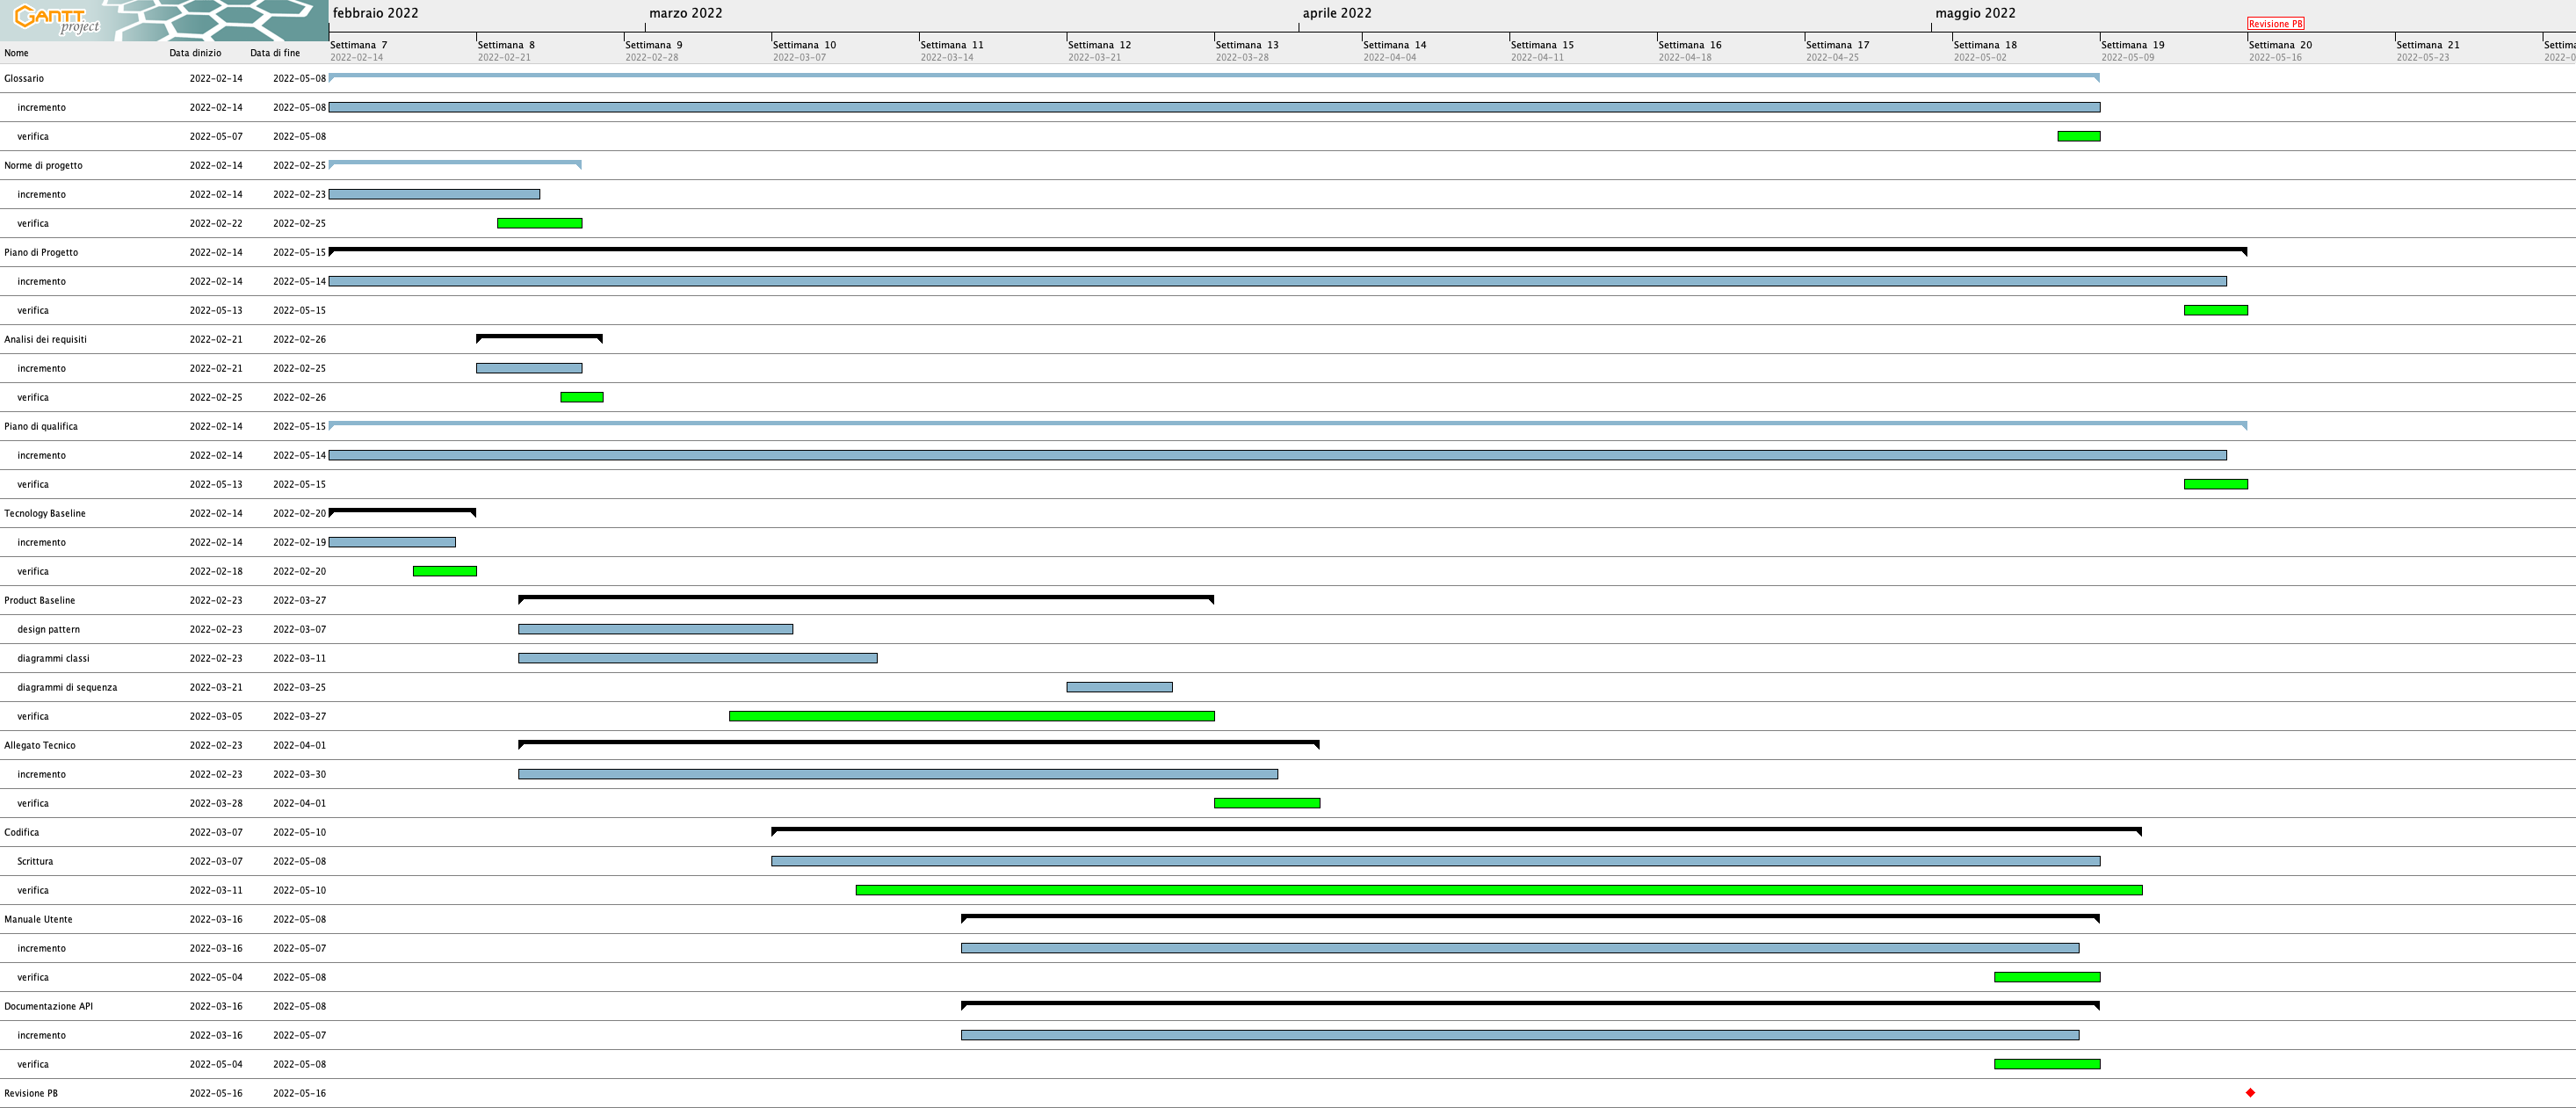
\includegraphics[scale=0.35]{Sezioni/gantt/progettazione_codifica.png}
\caption{Diagramma di Gantt - Progettazione e codifica}
\end{figure}